%%%%%%%%%%%%%%%%%%%%%%%%%%%%%%%%% Hauptteil %%%%%%%%%%%%%%%%%%%%%%%%%%%%%%%%%%

\chapter{Hauptteil}
\label{chap:Hauptteil}


\section{Beispiele}
Dies  ist eine Referenz auf ein Paper \cite{Kolter2009}. Die Verwaltung der Referenzen erfolgt in der Datei References.bib. Zur Bearbeitung der Referenzen kann beispielsweise das Programm JabRef\protect{\footnote{\url{http://jabref.sourceforge.net/}}} verwendet werden.

Besonders interessant ist auch die automatische Erstellung des Abkürzungsverzeichnisses. Zuerst wird die Abkürzung definiert um bei erstmaliger Verwendung im Abkürzungsverzeichnis zu erscheinen: \ac{Bsp.}, \ac{SaaS}

Referenzen auf Grafiken: \ref{fig:Fig1}, \ref{img:subFig2}, \ref{img:subFigs}

\begin{figure}
  \centering
  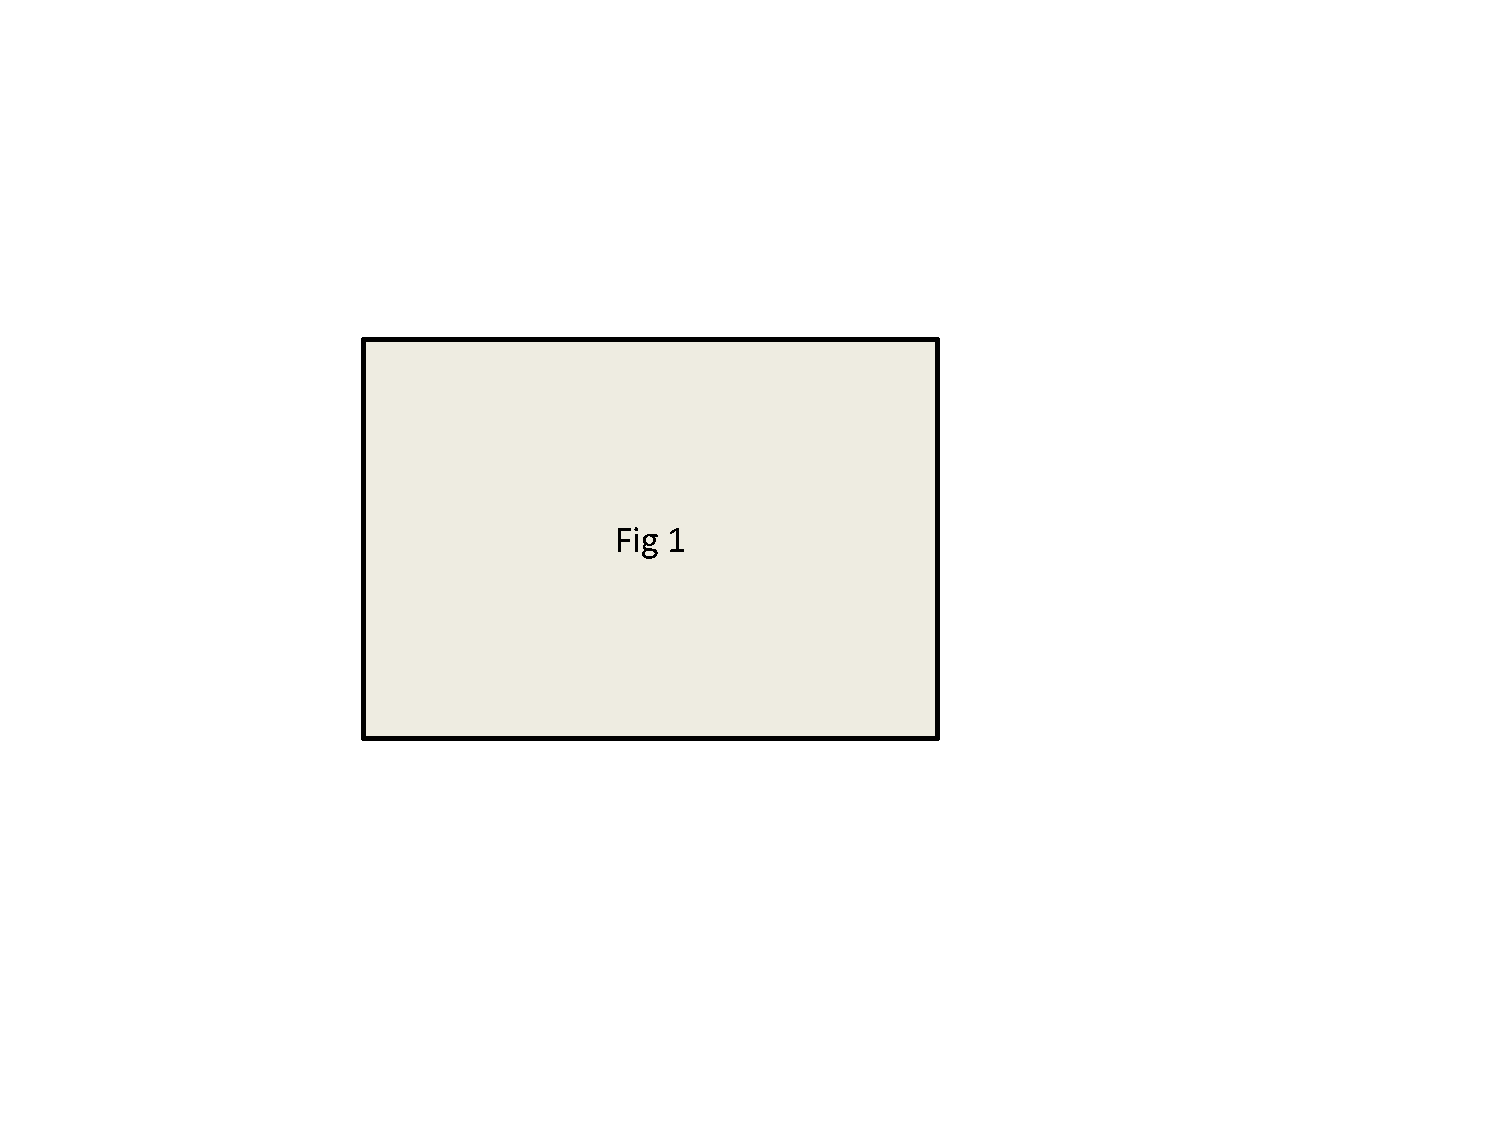
\includegraphics[width=0.95\textwidth]{Fig1.pdf}
  \caption{Beispielgrafik}
  \label{fig:Fig1}
\end{figure}


\begin{figure}
  \centering
  \subfigure[subfigure 1 \label{img:subFig1}]{\fbox{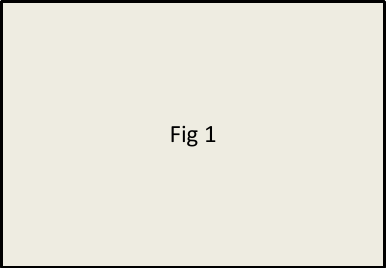
\includegraphics[width=0.45\textwidth]{Fig.png}}}\hfill
  \subfigure[subfigure 2\label{img:subFig2}]{\fbox{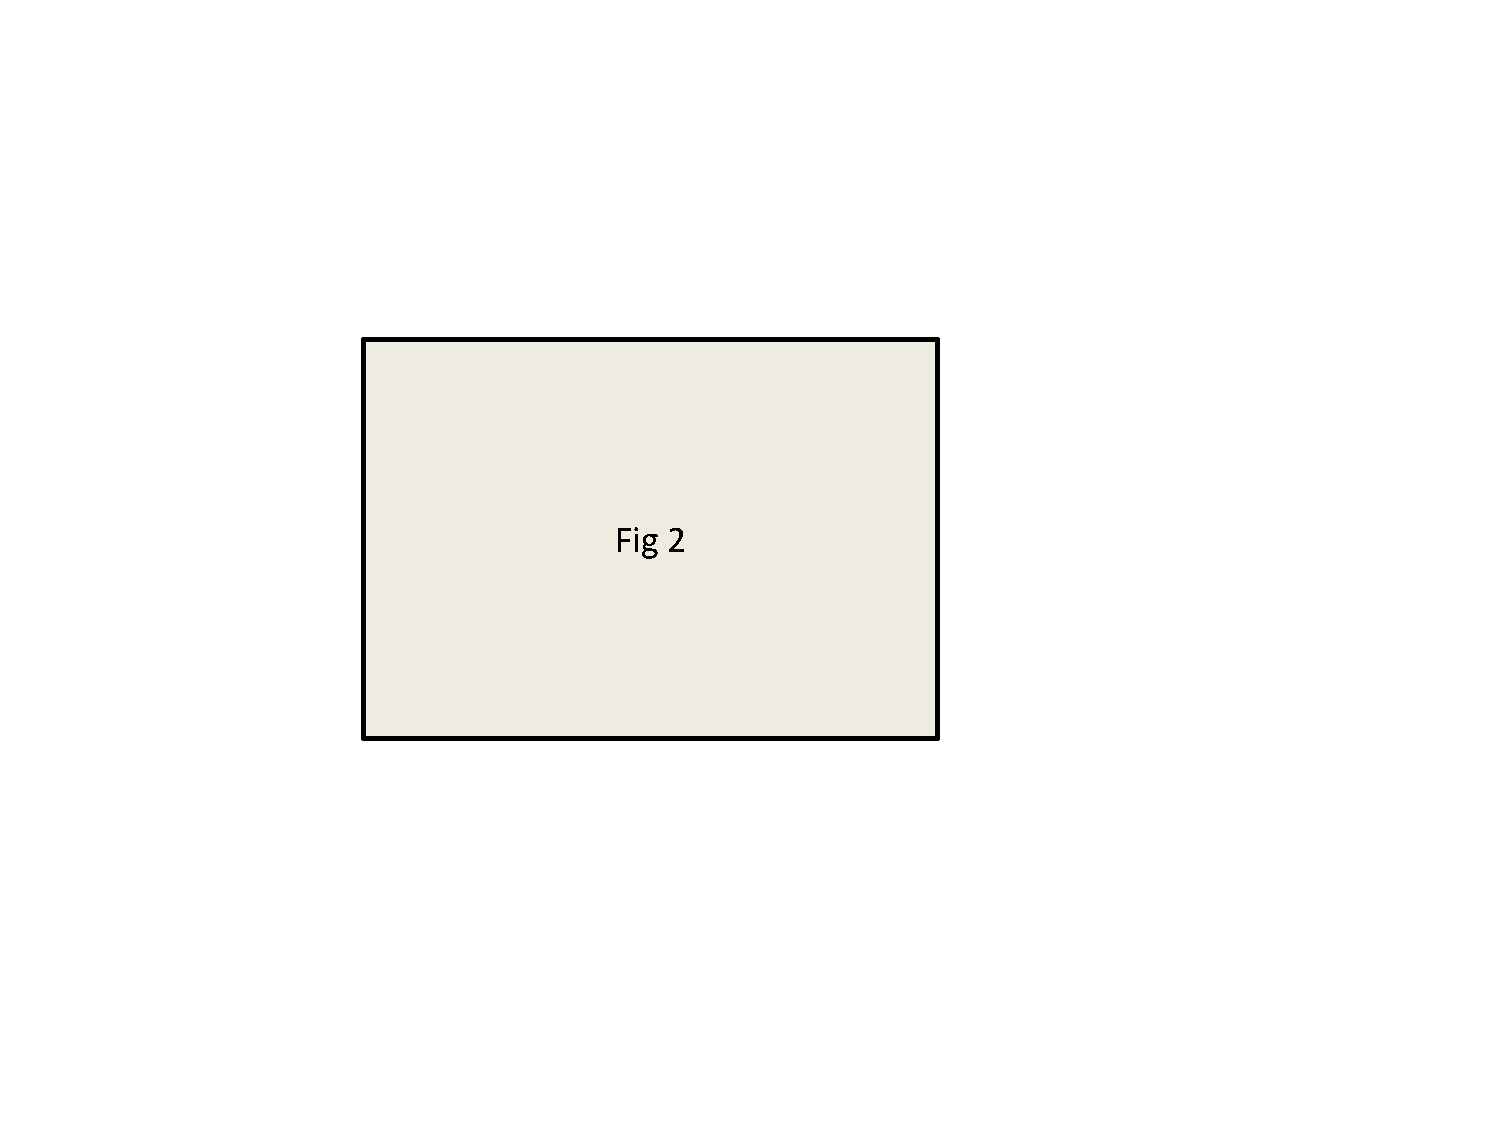
\includegraphics[width=0.45\textwidth]{Fig2.pdf}}}\hfill
  \caption{Beispiel subfigure}
  \label{img:subFigs}
\end{figure}



\lstset{language=JAVA, breaklines=true, tabsize=2}
\lstinputlisting[caption=HelloWorld,
label=lst:HelloWorld]{listings/HelloWorld.java}


%%%%%%%%%%%%%%%%%%%%%%%%%%%%%%%%%%%%%%%%%%%%%%%%%%%%%%%%%%%%%%%%%%%%%%%%%%%%%%
